\documentclass{beamer}
\usepackage{mstyle}
\usepackage{pgfplots}
\usepackage{appendixnumberbeamer}
\usetheme{Madrid}
\usefonttheme{serif}
\usetikzlibrary{intersections, pgfplots.fillbetween}
\setbeamertemplate{enumerate items}[default]
\makeatother
\setbeamertemplate{footline}
{
  \leavevmode%
  \hbox{%
  \begin{beamercolorbox}[wd=.2\paperwidth,ht=2.25ex,dp=1ex,center]{author in head/foot}%
    \usebeamerfont{author in head/foot}{Marco Vergamini}
  \end{beamercolorbox}%
  \begin{beamercolorbox}[wd=.55\paperwidth,ht=2.25ex,dp=1ex,center]{title in head/foot}%
    \usebeamerfont{title in head/foot}\insertshorttitle%\hspace*{3em}
  \end{beamercolorbox}%
  \begin{beamercolorbox}[wd=.25\paperwidth,ht=2.25ex,dp=1ex,center]{date in head/foot}%
    \usebeamerfont{date in head/foot}\insertshortdate\hspace*{1em}
    \insertframenumber{}/\inserttotalframenumber
  \end{beamercolorbox}}%
  \vskip0pt%
}
\makeatletter
\setbeamertemplate{navigation symbols}{}

\title{Teoremi di tipo ``Wolff-Denjoy'' in più variabili complesse}
\institute{Università di Pisa \\
Corso di Laurea Triennale in Matematica}
\date{22 Settembre 2023 (realisticamente)}
\titlegraphic{
\includegraphics[width=0.30\textwidth]{Stemma_unipi.jpg}}
\author{Candidato: Marco Vergamini \qquad Relatore: Prof. Marco Abate}

\begin{document}

\begin{frame}
  \begin{beamercolorbox}[sep=8pt,center,colsep=-4bp,rounded=true,shadow=true]{title}
    \usebeamerfont{title}\inserttitle\par%
    \ifx\insertsubtitle\@empty%
    \else%
    \vskip0.25em%
    {\usebeamerfont{subtitle}\usebeamercolor[fg]{subtitle}\insertsubtitle\par}%
    \fi%
  \end{beamercolorbox}

  \begin{beamercolorbox}[sep=8pt,center,colsep=-4bp,rounded=true,shadow=true]{date}
    \usebeamerfont{date}\insertdate
  \end{beamercolorbox}\vskip0.5em

  \begin{center}
    {\usebeamercolor[fg]{titlegraphic}\inserttitlegraphic\par}
  \end{center}

  \begin{beamercolorbox}[sep=8pt,center,colsep=-4bp,rounded=true,shadow=true]{institute}
    \usebeamerfont{institute}\insertinstitute
  \end{beamercolorbox}

  \begin{beamercolorbox}[sep=8pt,center,colsep=-4bp,rounded=true,shadow=true]{author}
    \usebeamerfont{author}\insertauthor
  \end{beamercolorbox}
\end{frame}

\begin{frame}
  \frametitle{Il teorema di Wolff-Denjoy}
  Sia $\mathbb{D}$ il disco unitario in $\mathbb{C}$.\pause
  \begin{block}{Teorema (Wolff-Denjoy, 1926)}
    \begin{itshape}
      Sia $f:\mathbb{D} \longrightarrow \mathbb{D}$ una funzione olomorfa. \pause Allora vale esattamente una delle seguenti affermazioni:\pause
      \begin{itemize}
        \item la funzione $f$ ha un punto fisso nel disco; \pause oppure,
        \item esiste un unico punto del bordo del disco tale che la successione delle iterate di $f$ converge, uniformemente sui compatti, a quel punto.
      \end{itemize}
    \end{itshape}
  \end{block}
\end{frame}

\begin{frame}[t]
  \frametitle{Generalizzazione ai domini limitati e strettamente pseudoconvessi}
  \only<1>{
    \begin{defn}
      La \textit{distanza di Poincaré} (o \textit{iperbolica}) $\omega$ su $\mathbb{D}$ è data da
      \begin{equation*}
          \omega(z_1,z_2)=\frac{1}{2}\log{\frac{1+\left|\frac{z_1-z_2}{1-\bar{z}_1z_2}\right|}{1-\left|\frac{z_1-z_2}{1-\bar{z}_1z_2}\right|}}
      \end{equation*}
      per ogni $z_1,z_2 \in \mathbb{D}$.
  \end{defn}
  }
  \only<2-3>{
    \begin{defn}
      Sia $X$ una varietà complessa e connessa; la \textit{pseudodistanza di Kobayashi} su $X$ è data da
    \begin{equation*}\begin{split}
        k_X(z,w)=&\inf\Bigg\{\sum_{j=1}^m \omega(\zeta_{j-1},\zeta_j) \bigg\vert \text{esistono }m\in\mathbb{N},\text{ punti }\zeta_0,\dots,\zeta_m \in \mathbb{D}\text{ e}\\
        &\text{funzioni }\varphi_1,\dots,\varphi_m\in\text{Hol}(\mathbb{D},X) \text{ tali che } \varphi_1(\zeta_0)=z,\\
        &\varphi_m(\zeta_m)=w\text{ e }\varphi_j(\zeta_j)=\varphi_{j+1}(\zeta_j)\text{ per }j=1,\dots,m-1\Bigg\}
    \end{split}\end{equation*}
    per $z,w \in X$.
    
    \setcounter{beamerpauses}{2}\pause Se $k_X$ è una distanza, diremo che $X$ è \textit{Kobayashi-iperbolica}.
    \end{defn}
  }
  \only<4-7>{
    \begin{defn}
      Sia $\Omega \subseteq \mathbb{C}^n, n \ge 2$ un dominio limitato con bordo $C^2$, cioè esiste una \textit{funzione di definizione} $\rho \in C^2(\mathbb{C}^n)$ tale che $\Omega=\{\rho(z)<0\}$ e $\diff\rho\not=0$ in ogni punto di $\partial\Omega$. \setcounter{beamerpauses}{4}\pause Dato $p \in \partial\Omega$, lo \textit{spazio tangente complesso} a $\partial\Omega$ in $p$ è $H_p\partial\Omega=\{Z \in \mathbb{C}^n \mid \langle \bar{\partial}\rho(p),Z\rangle=0\}$. \pause Diciamo che $\Omega$ è \textit{strettamente pseudoconvesso in $p$} se la \textit{forma di Levi}
      $$L_{\rho}(p;Z)=\sum_{\nu,\mu=1}^n \frac{\partial^2\rho}{\partial z_\nu\partial\bar{z}_\mu}(p)Z_\nu\bar{Z}_\mu, \quad Z=(Z_1,\dots,Z_n) \in \mathbb{C}^n$$
      è definita positiva in $H_p\partial\Omega$.\pause

      Diciamo che $\Omega$ è \textit{strettamente pseudoconvesso} se è strettamente pseudoconvesso in $p$ per ogni $p \in \partial\Omega$.
    \end{defn}
  }
  \only<8->{
  \begin{block}{Teorema (Abate, 1991)}\begin{itshape}
    Siano $\Omega\subseteq\mathbb{C}^n$ un dominio limitato e strettamente pseudoconvesso e $f:\Omega \longrightarrow \Omega$ una funzione olomorfa. \setcounter{beamerpauses}{8}\pause Allora vale esattamente una delle seguenti affermazioni: \pause
    \begin{enumerate}
      \item le orbite di $f$ sono relativamente compatte in $\Omega$; \pause oppure,
      \item esiste un unico punto di $\partial\Omega$ tale che le iterate di $f$ convergono tutte, uniformemente sui compatti, a quel punto.
    \end{enumerate}
  \end{itshape}\end{block}}\only<12->{
    \textit{Traccia della dimostrazione:} Per un teorema di Balogh e Bonk del 2000, $(\Omega,k_\Omega)$ è uno spazio metrico Gromov-iperbolico. \only<13->{

    Allora soddisfa le ipotesi di un teorema di Karlsson del 2001, per cui le orbite sono limitate (in $k_\Omega$) o convergono a un unico punto del bordo.} \only<14->{

    Per avere la convergenza uniforme sui compatti si applica il teorema di Montel. \qed}
  }
\end{frame}

\begin{frame}[t]
  \frametitle{La condizione di visibilità}
  \only<1-2>{
    \begin{defn}
      Sia $X$ una varietà complessa; la \textit{pseudometrica di Kobayashi} su $X$ è
      \begin{equation*}\begin{split}
          K_X(x;Z)=&\inf\{|v| \mid v \in \mathbb{C}, \text{ esiste }f \in \text{Hol}(\mathbb{D},X) \\
          &\text{ tale che } f(0)=x, \diff_0 f(v)=Z\}
      \end{split}\end{equation*}
      per ogni $x \in X$ e $Z \in T_xX$.
    \end{defn}
  }
  \only<2>{
    Le funzioni olomorfe sono semicontrazioni sia rispetto a $K_X$ che rispetto a $k_X$.
  }
  \only<3-6>{
    \begin{defn}
      Sia $X$ una varietà complessa e connessa; fissiamo due costanti $\lambda \ge 1$ e $\kappa \ge 0$. Sia $I\subseteq \mathbb{R}$ un intervallo; \setcounter{beamerpauses}{3}\pause una curva $\sigma:I \longrightarrow X$ è detta una \textit{$(\lambda,\kappa)$-simil-geodetica} se:\pause
    \begin{enumerate}
        \item per ogni $s,t \in I$ si ha
        \begin{equation*}
            \frac{1}{\lambda}|t-s|-\kappa \le k_X\big(\sigma(s),\sigma(t)\big)\le\lambda|t-s|+\kappa;
        \end{equation*}\pause
        \item $\sigma$ è assolutamente continua rispetto a $d_X$ (quindi $\sigma'(t)$ esiste per quasi ogni $t \in I$) e per quasi ogni $t \in I$ si ha
        \begin{equation*}
            K_X\big(\sigma(t);\sigma'(t)\big) \le \lambda.
        \end{equation*}
    \end{enumerate}
    \end{defn}
  }
  \only<7-10>{
    \begin{defn}
      Sia $X$ una sottovarietà complessa e connessa di una varietà complessa $Y$, e fissiamo $\lambda \ge 1$ e $\kappa \ge 0$. \setcounter{beamerpauses}{7}\pause Diciamo che $X$ è \textit{$(\lambda,\kappa)$-visibile} se:\pause
      \begin{enumerate}
          \item ogni due punti distinti di $X$ possono essere collegati da una $(\lambda,\kappa)$-simil-geodetica;\pause
          \item per ogni coppia di punti $p,q\in\partial_YX$ con $p\not=q$, esistono in $\overline{X}$ due intorni $V$ e $W$, di $p$ e $q$ rispettivamente, con chiusura disgiunta, e un compatto $K$ di $X$ tali che  ogni $(\lambda,\kappa)$-simil-geodetica in $X$ che collega un punto di $V$ a un punto di $W$ interseca $K$.
      \end{enumerate}
  \end{defn}
  }
  \only<11-15>{
    Caso escluso: le simil-geodetiche da $U$ a $V$ fuggono dal compatto $K$.
  }
  \only<11>{
    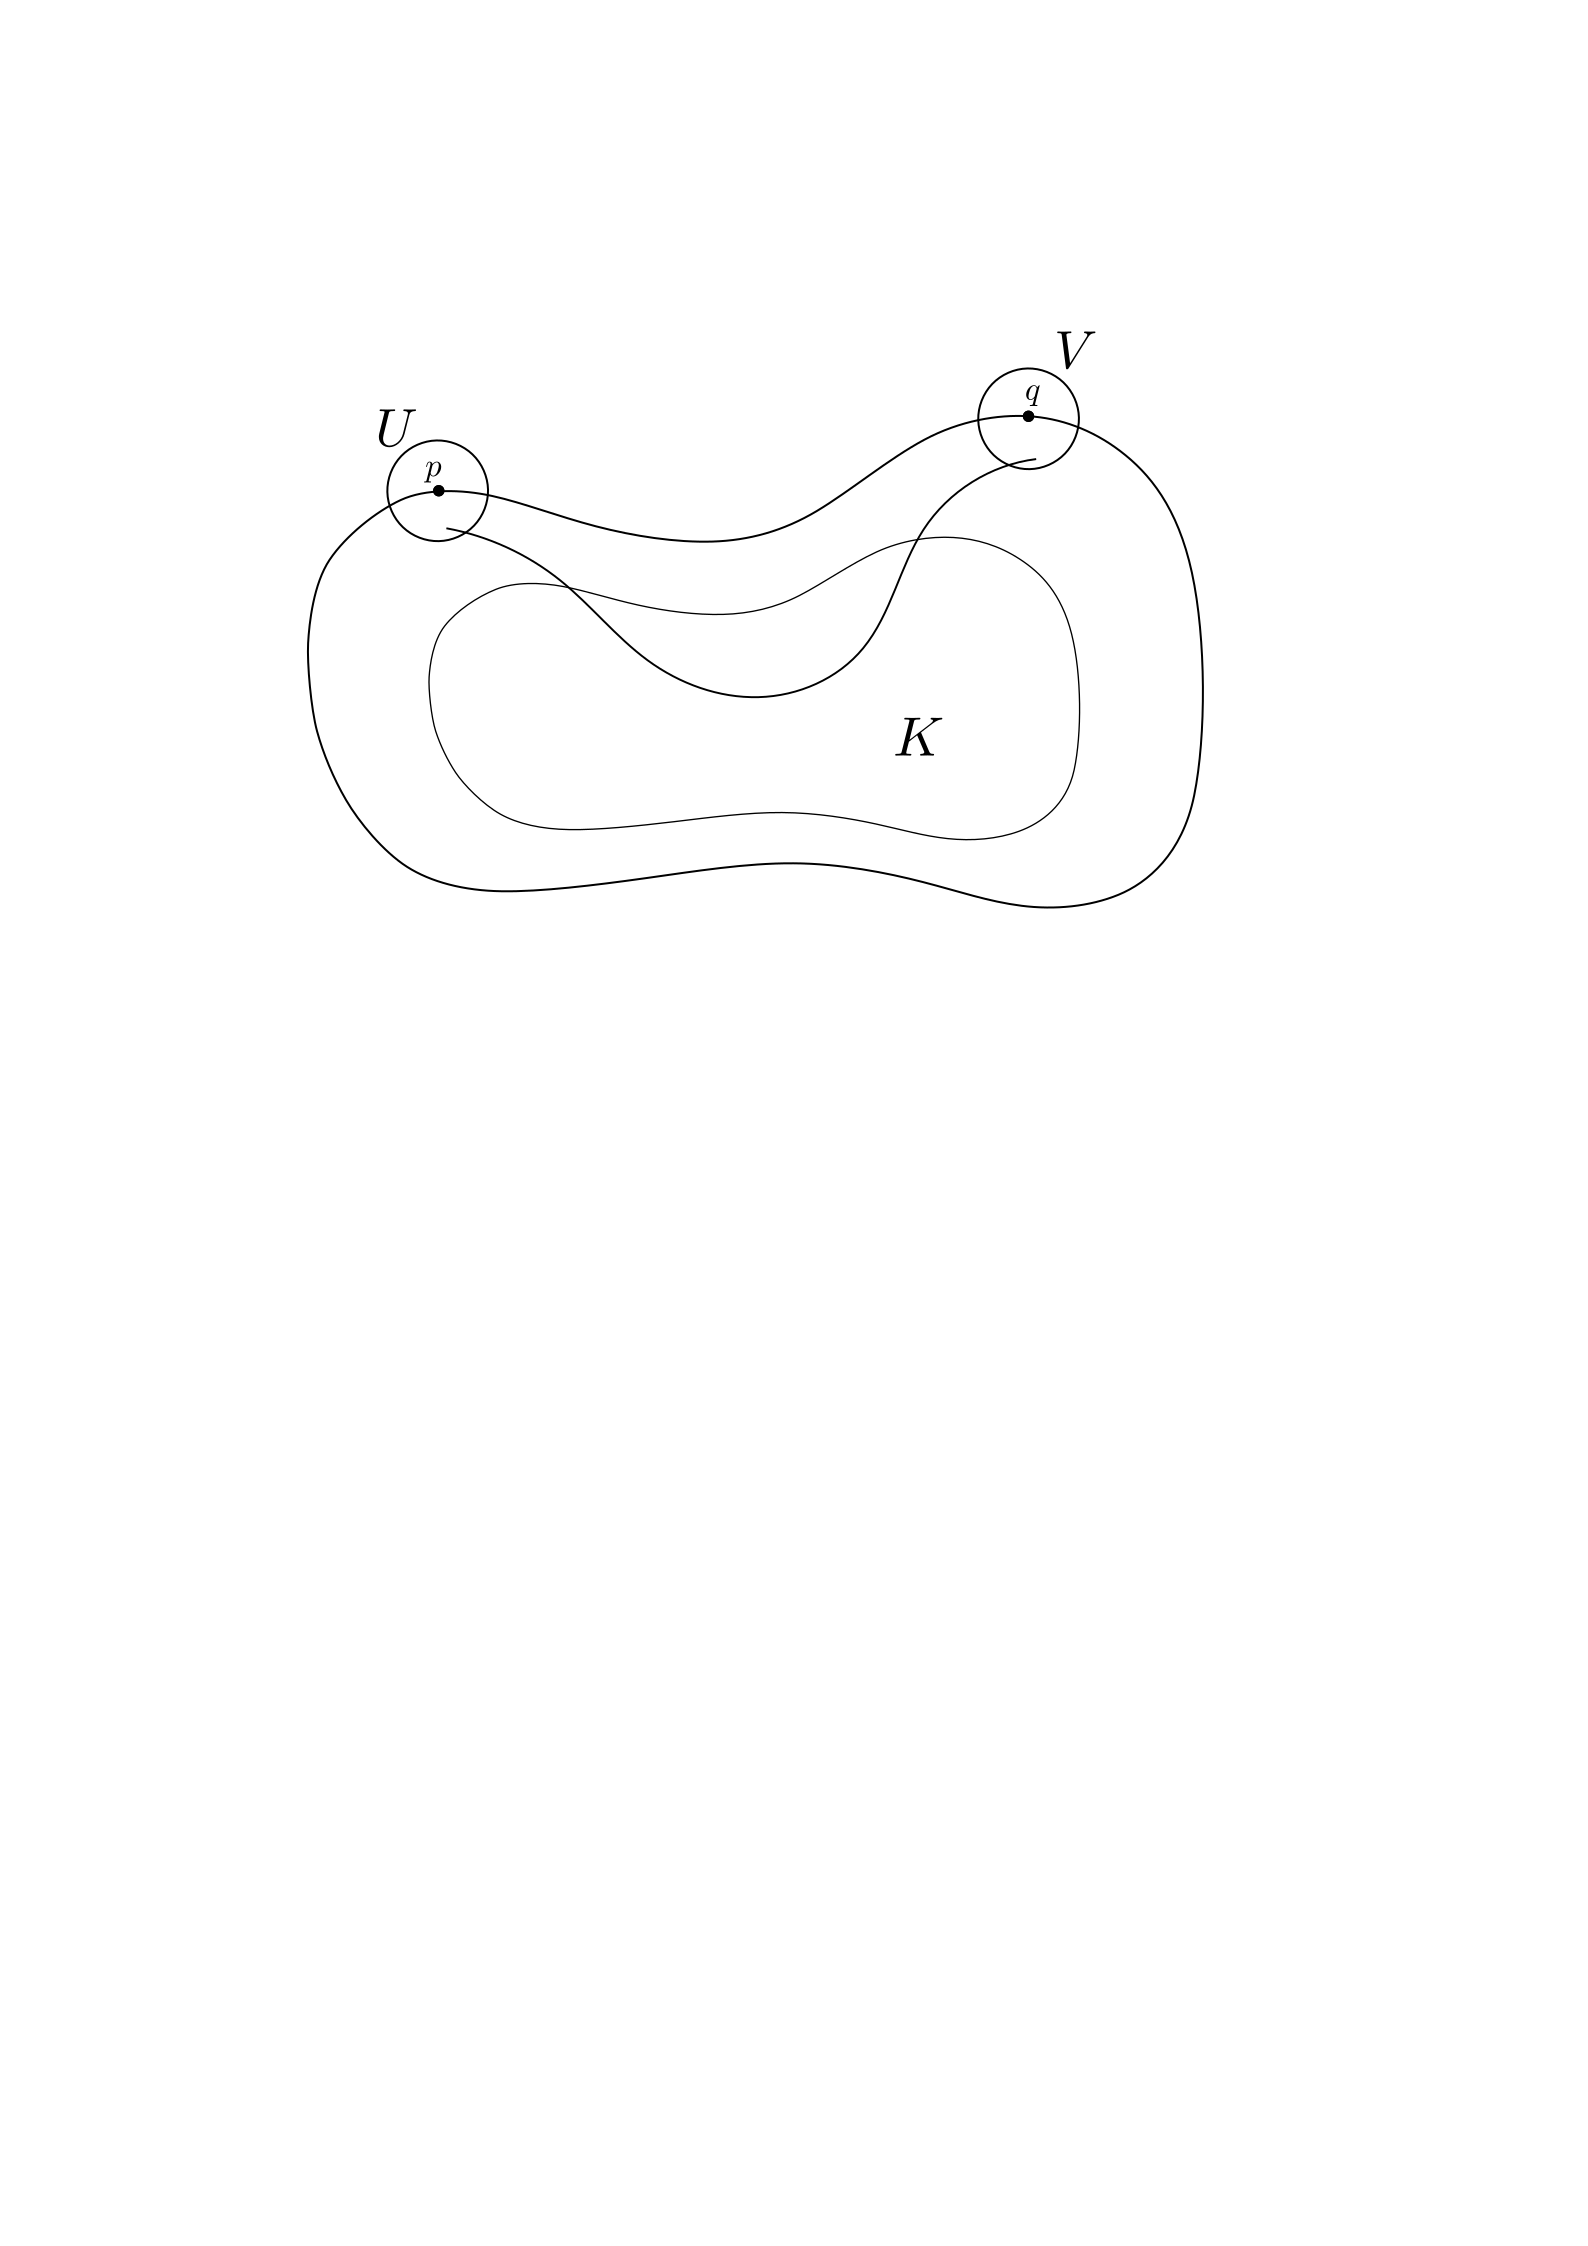
\includegraphics[width=1.05\textwidth, trim=0 18cm 0 3cm]{vis1.png}
  }
  \only<12>{
    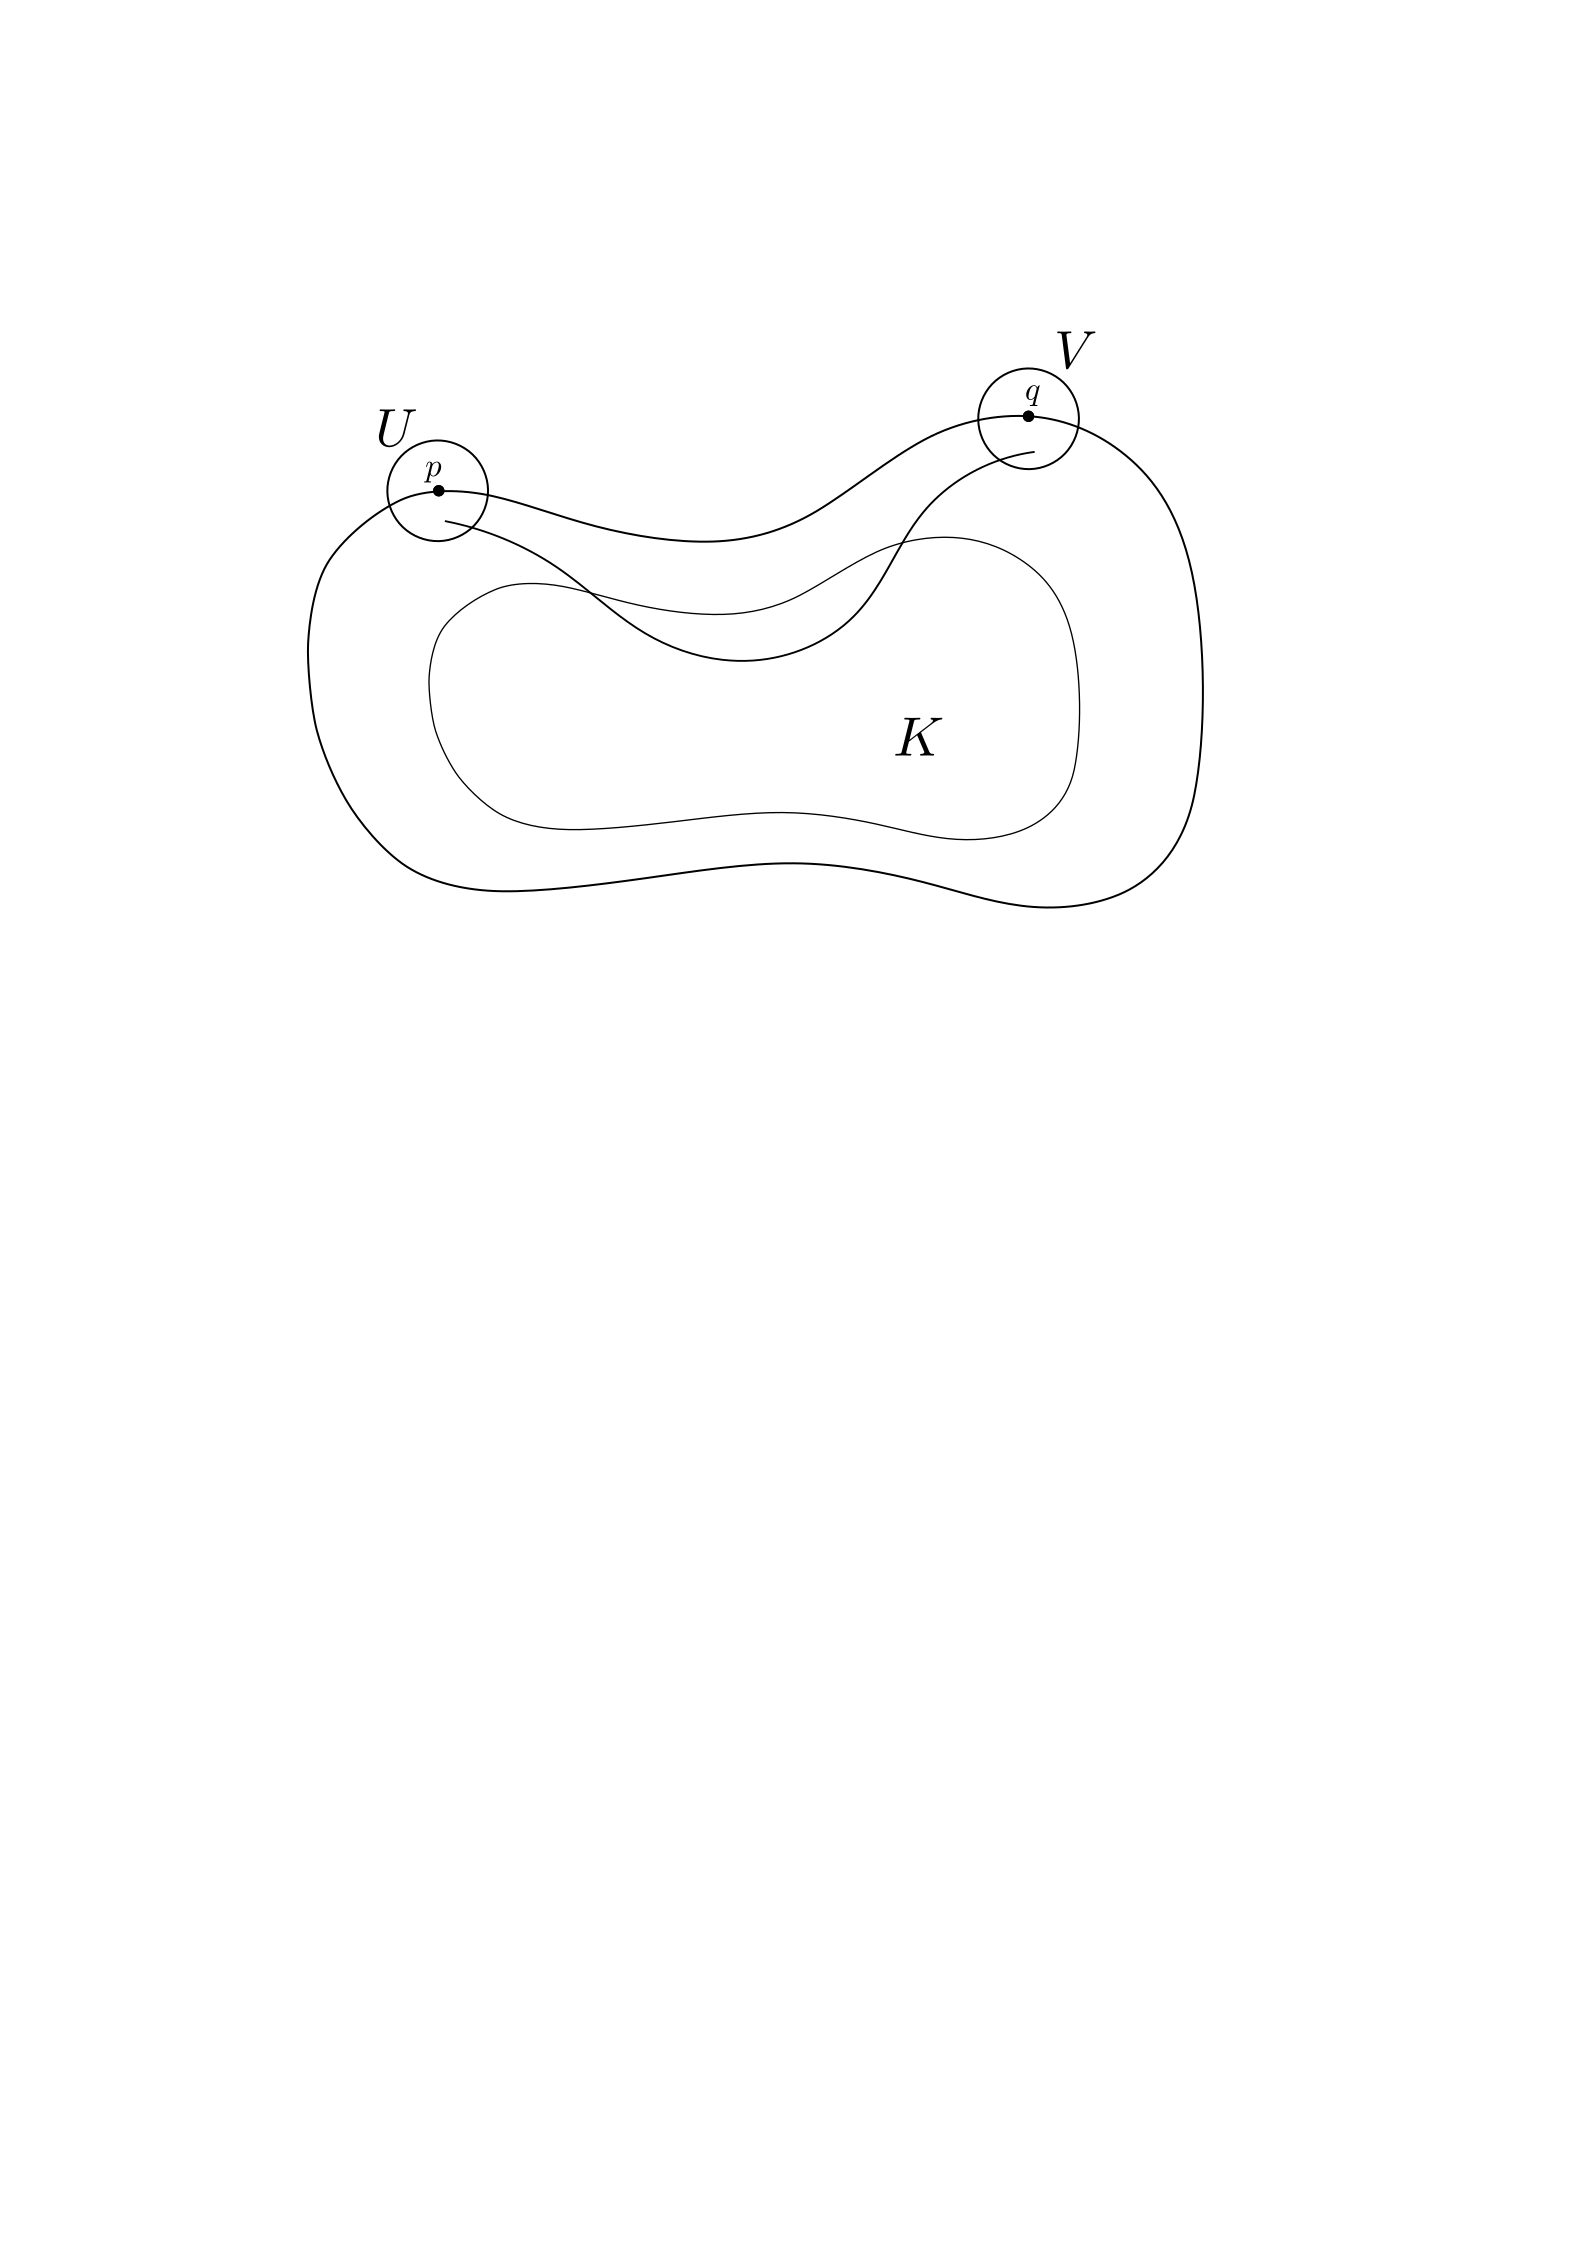
\includegraphics[width=1.05\textwidth, trim=0 18cm 0 3cm]{vis2.png}
  }
  \only<13>{
    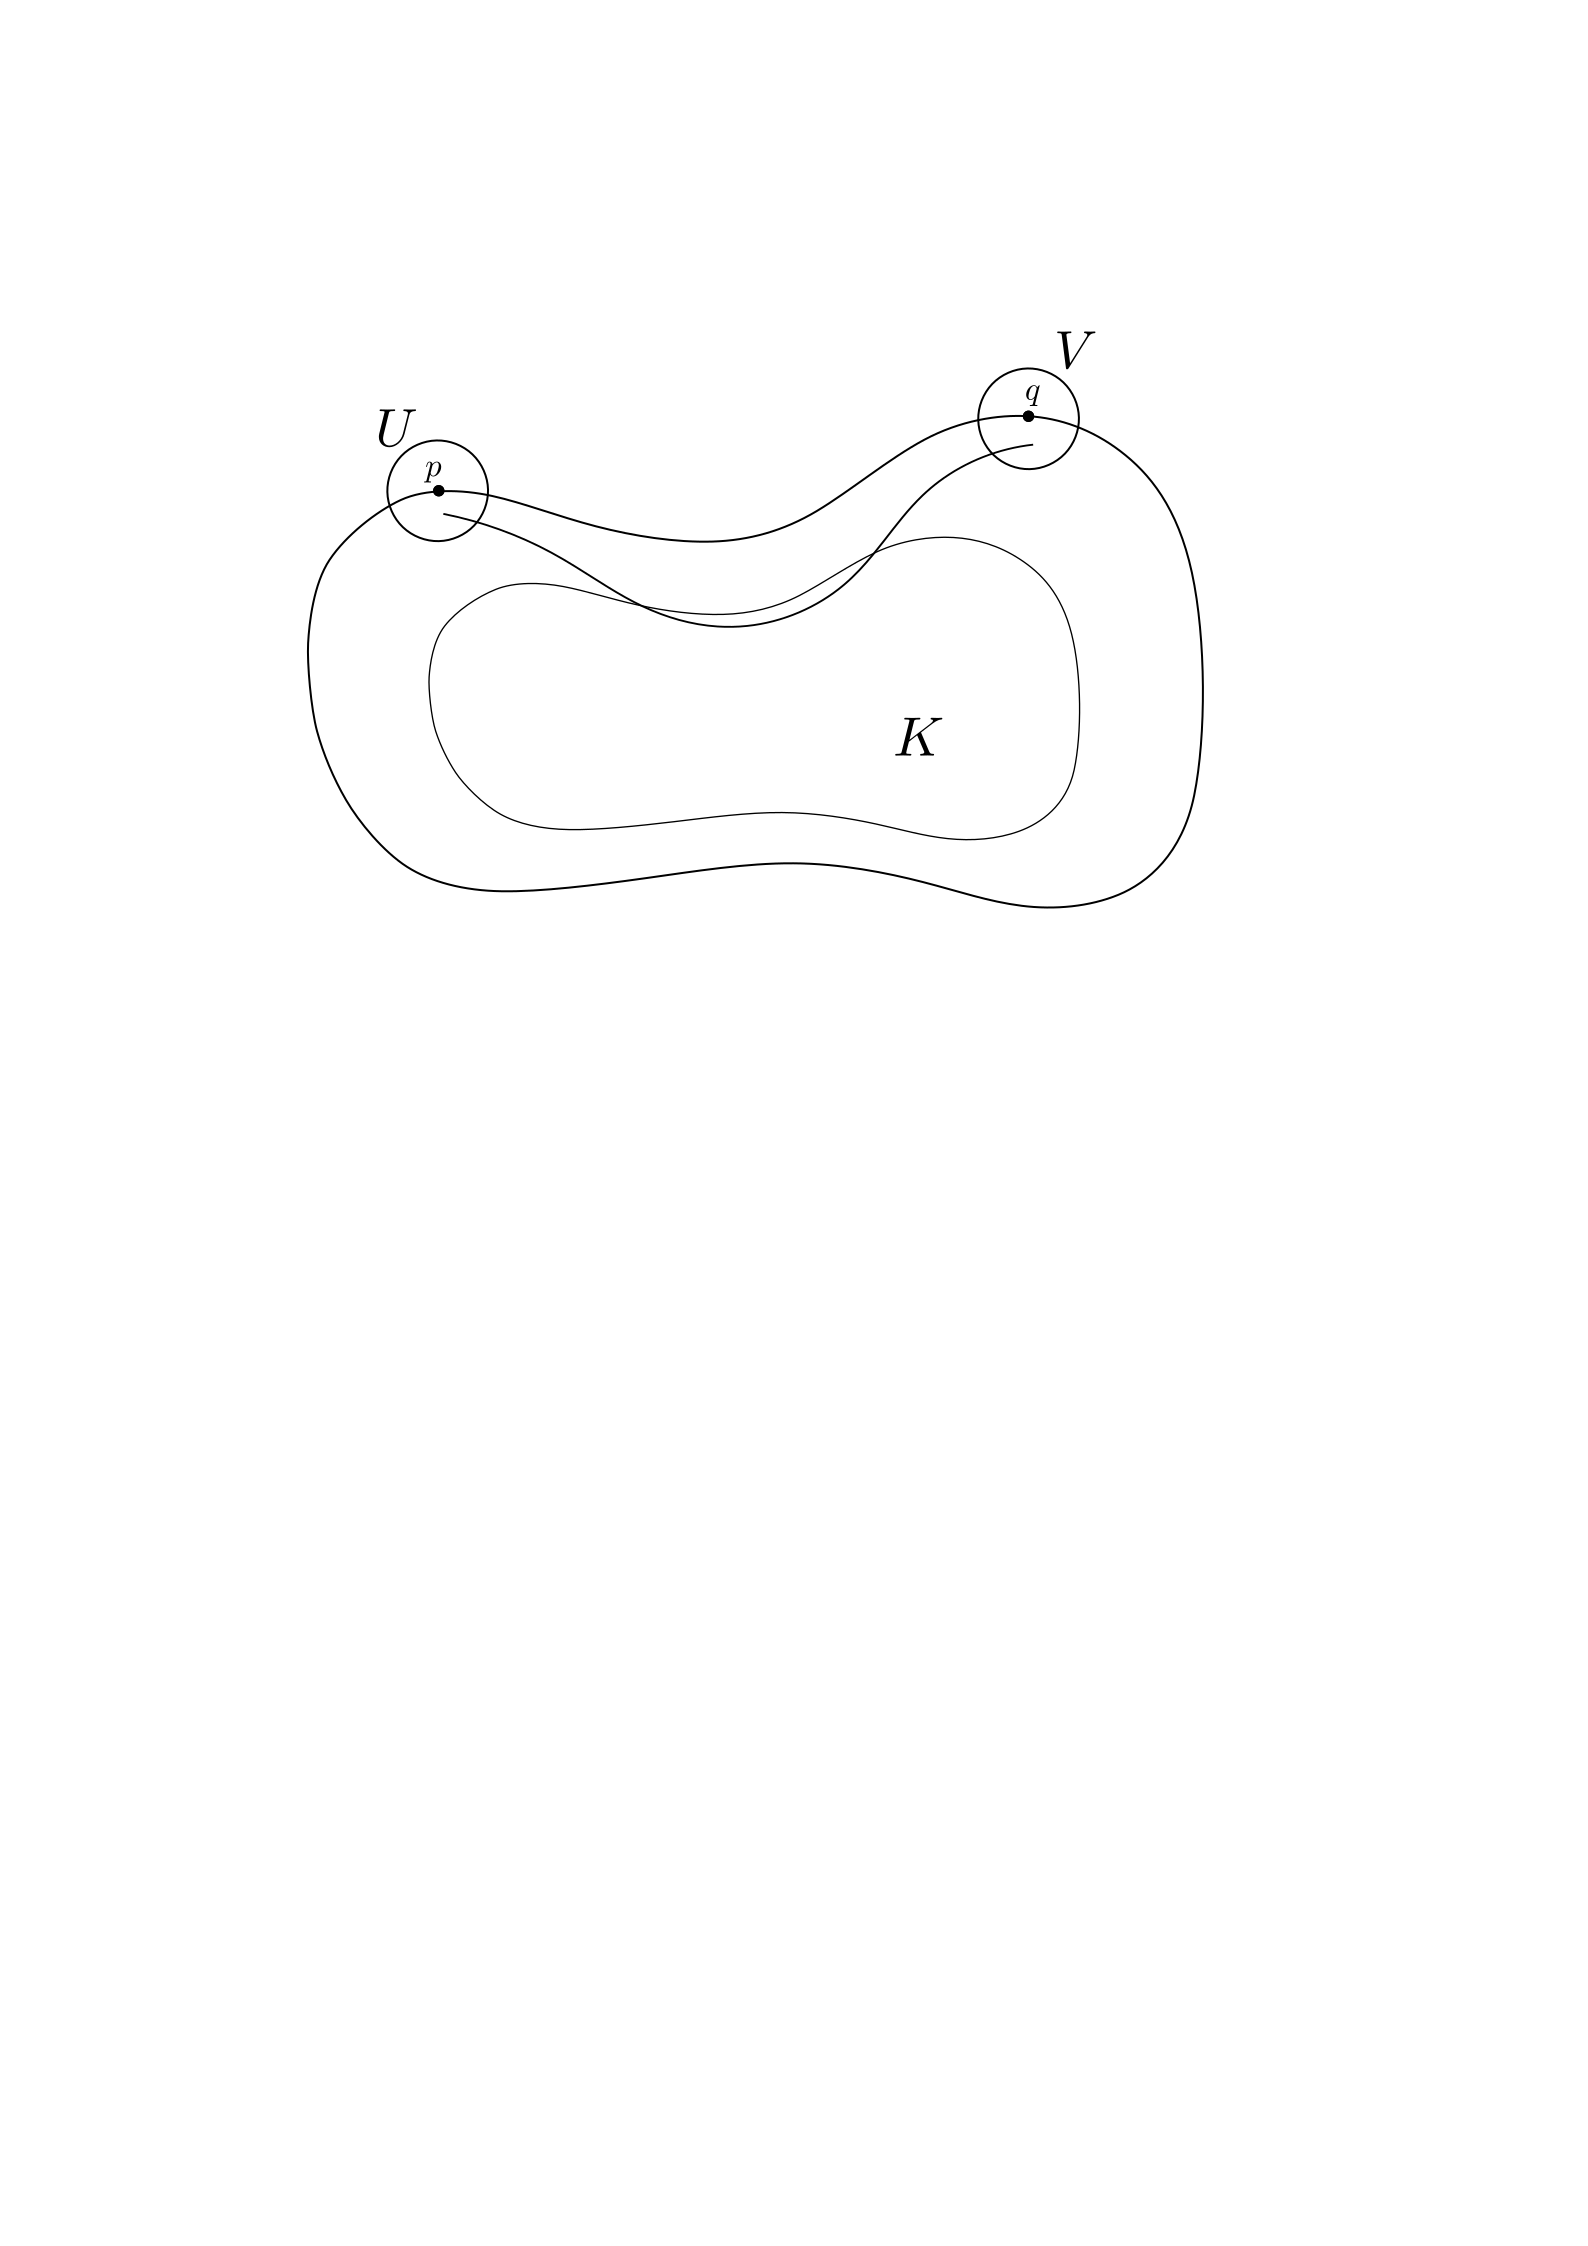
\includegraphics[width=1.05\textwidth, trim=0 18cm 0 3cm]{vis3.png}
  }
  \only<14>{
    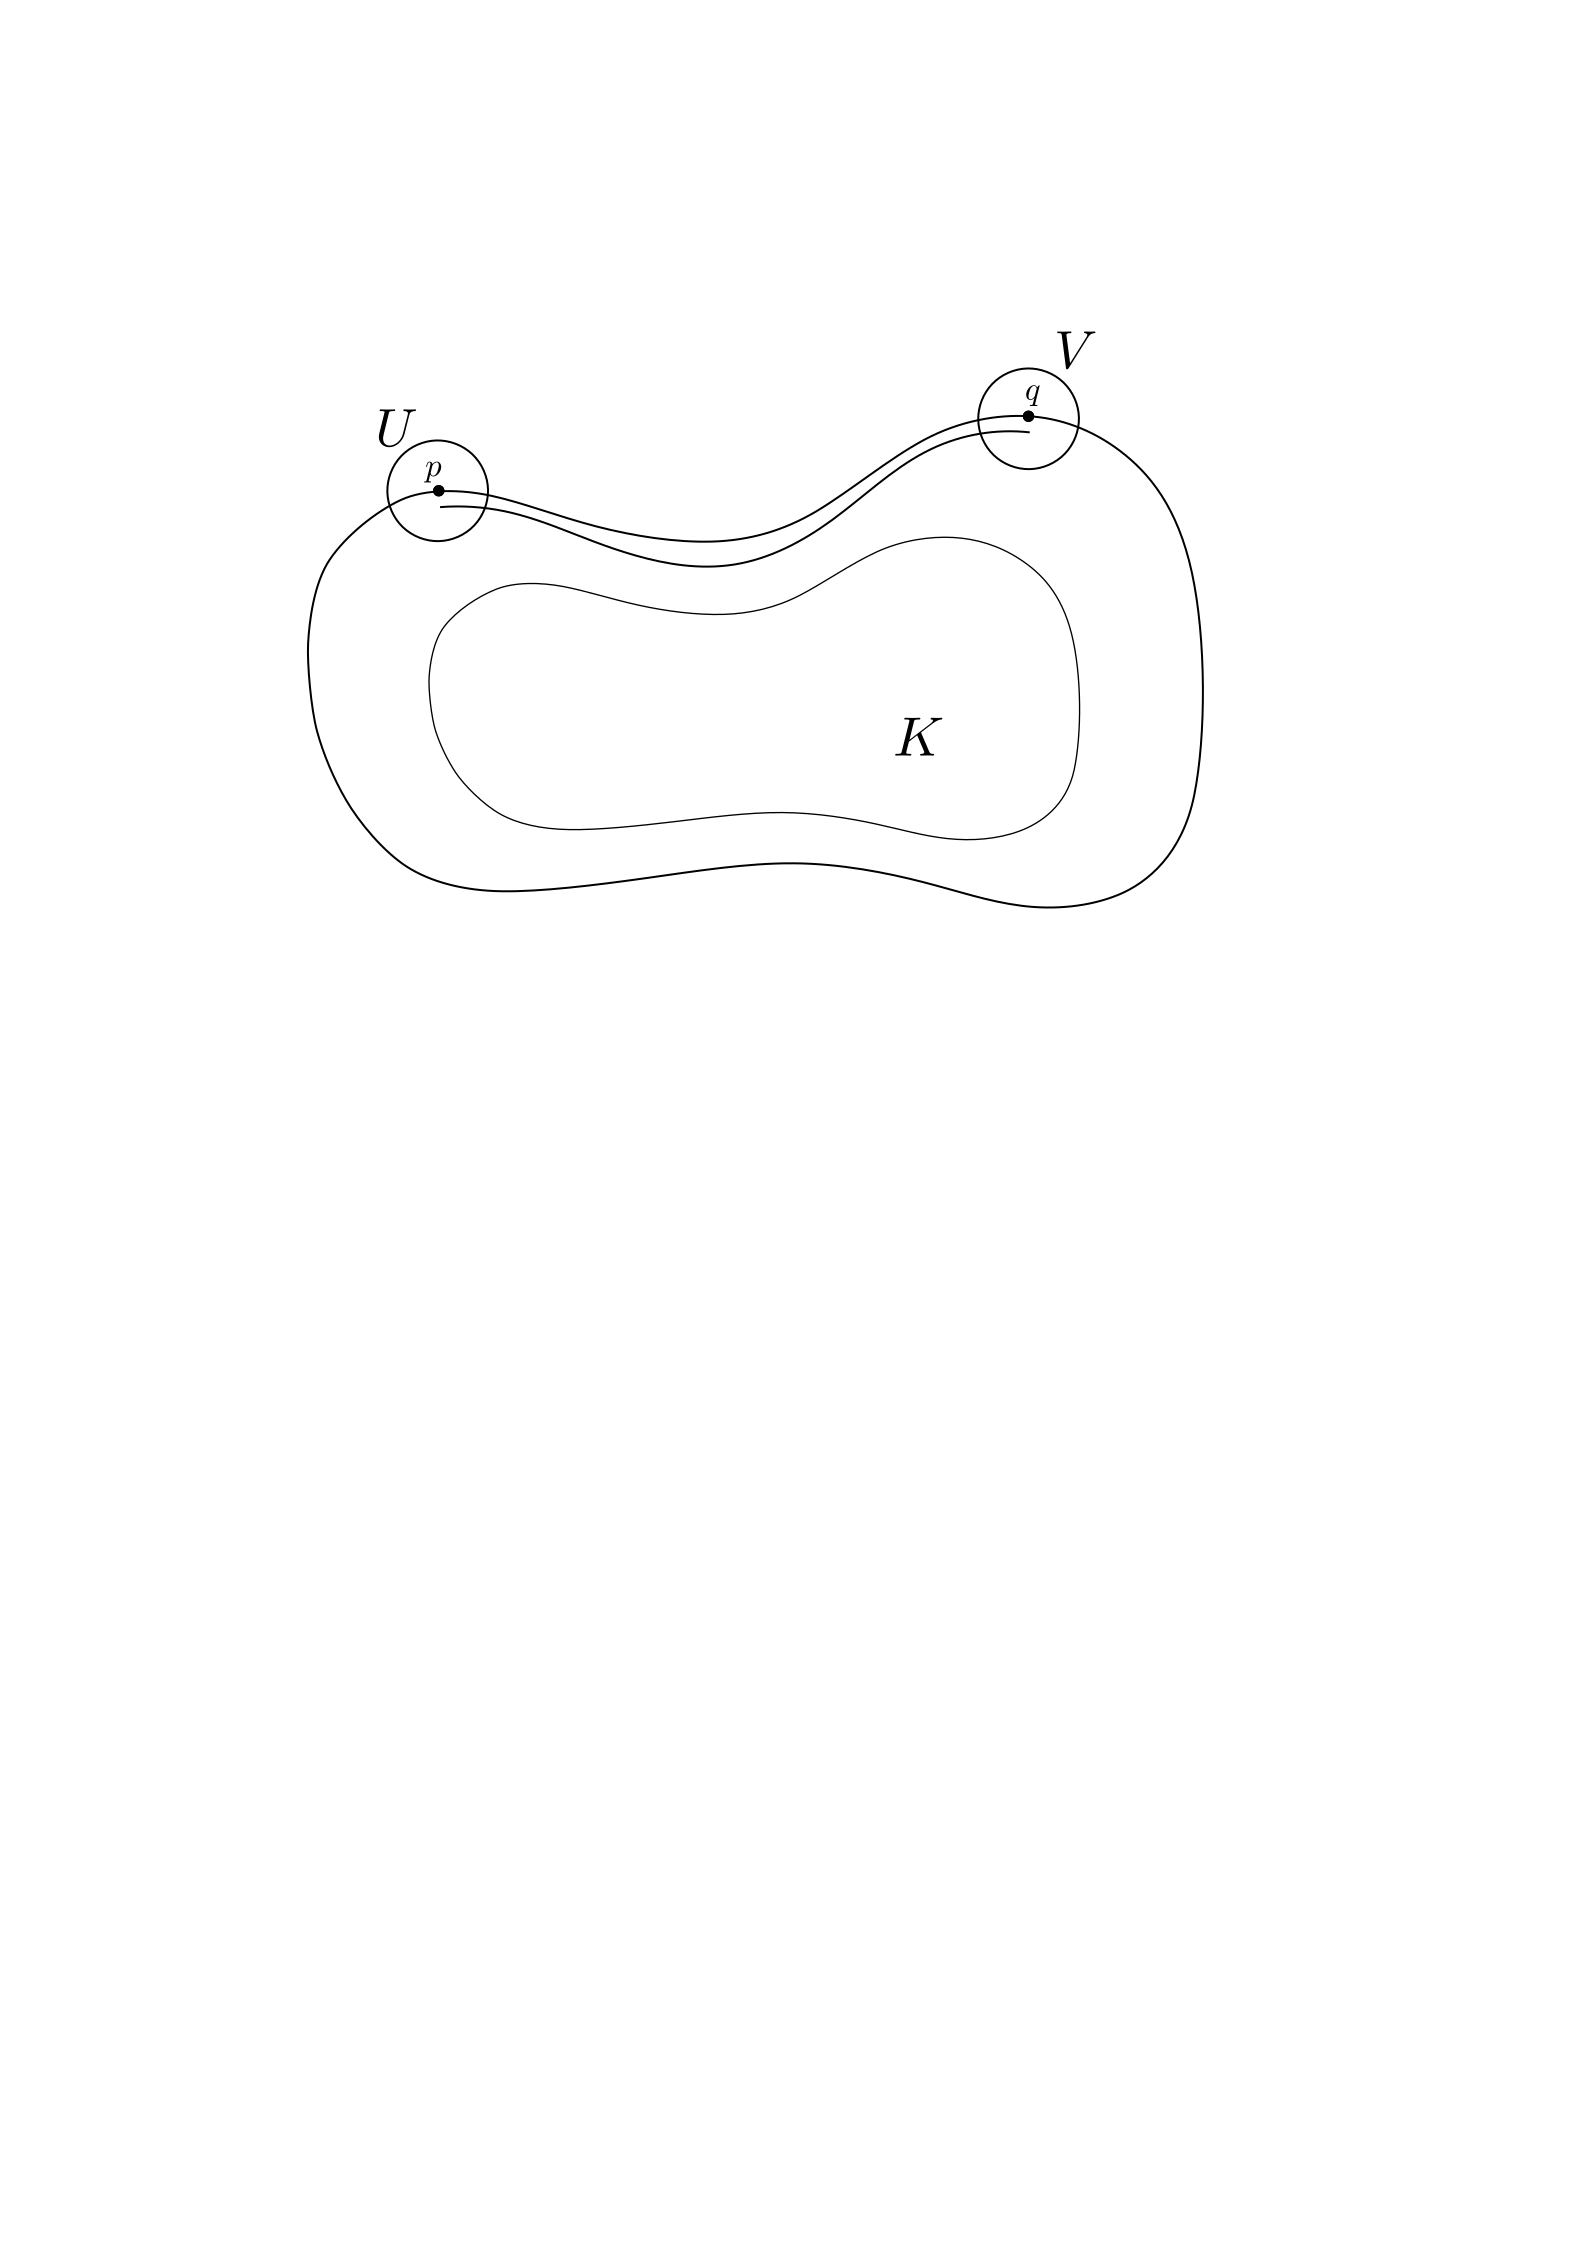
\includegraphics[width=1.05\textwidth, trim=0 18cm 0 3cm]{nonvis4.png}
  }
  \only<15>{
    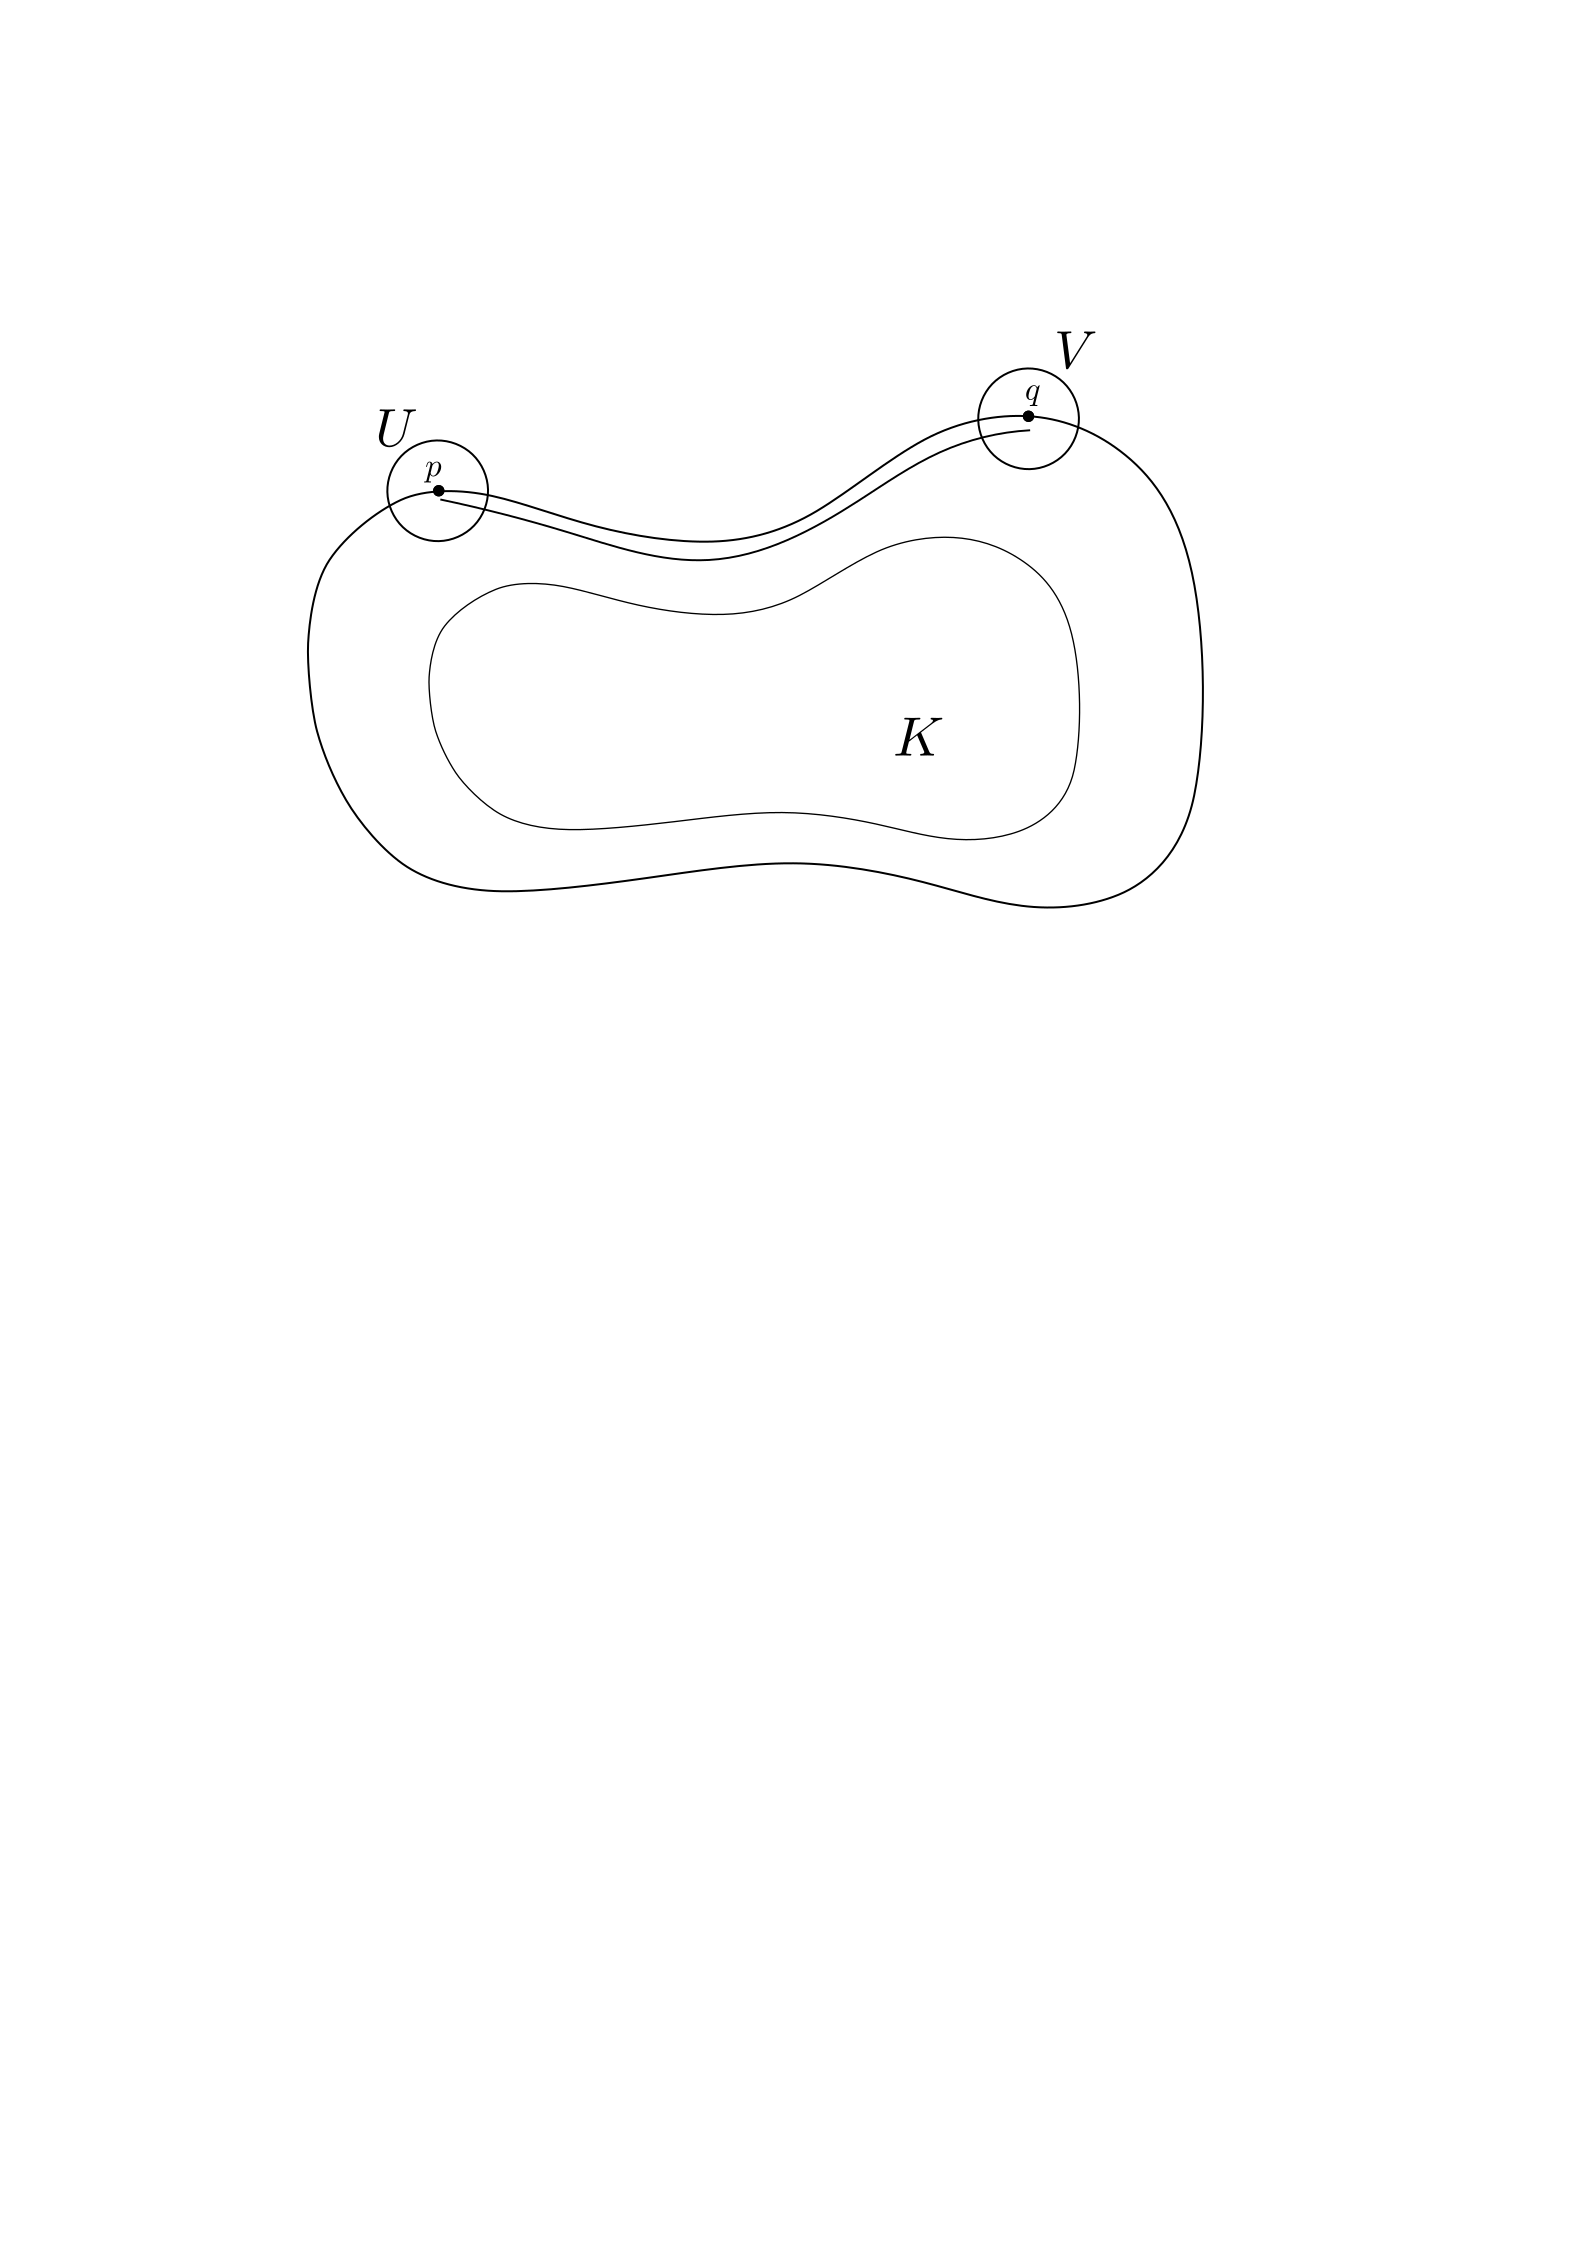
\includegraphics[width=1.05\textwidth, trim=0 18cm 0 3cm]{nonvis5.png}
  }
  \only<16>{
    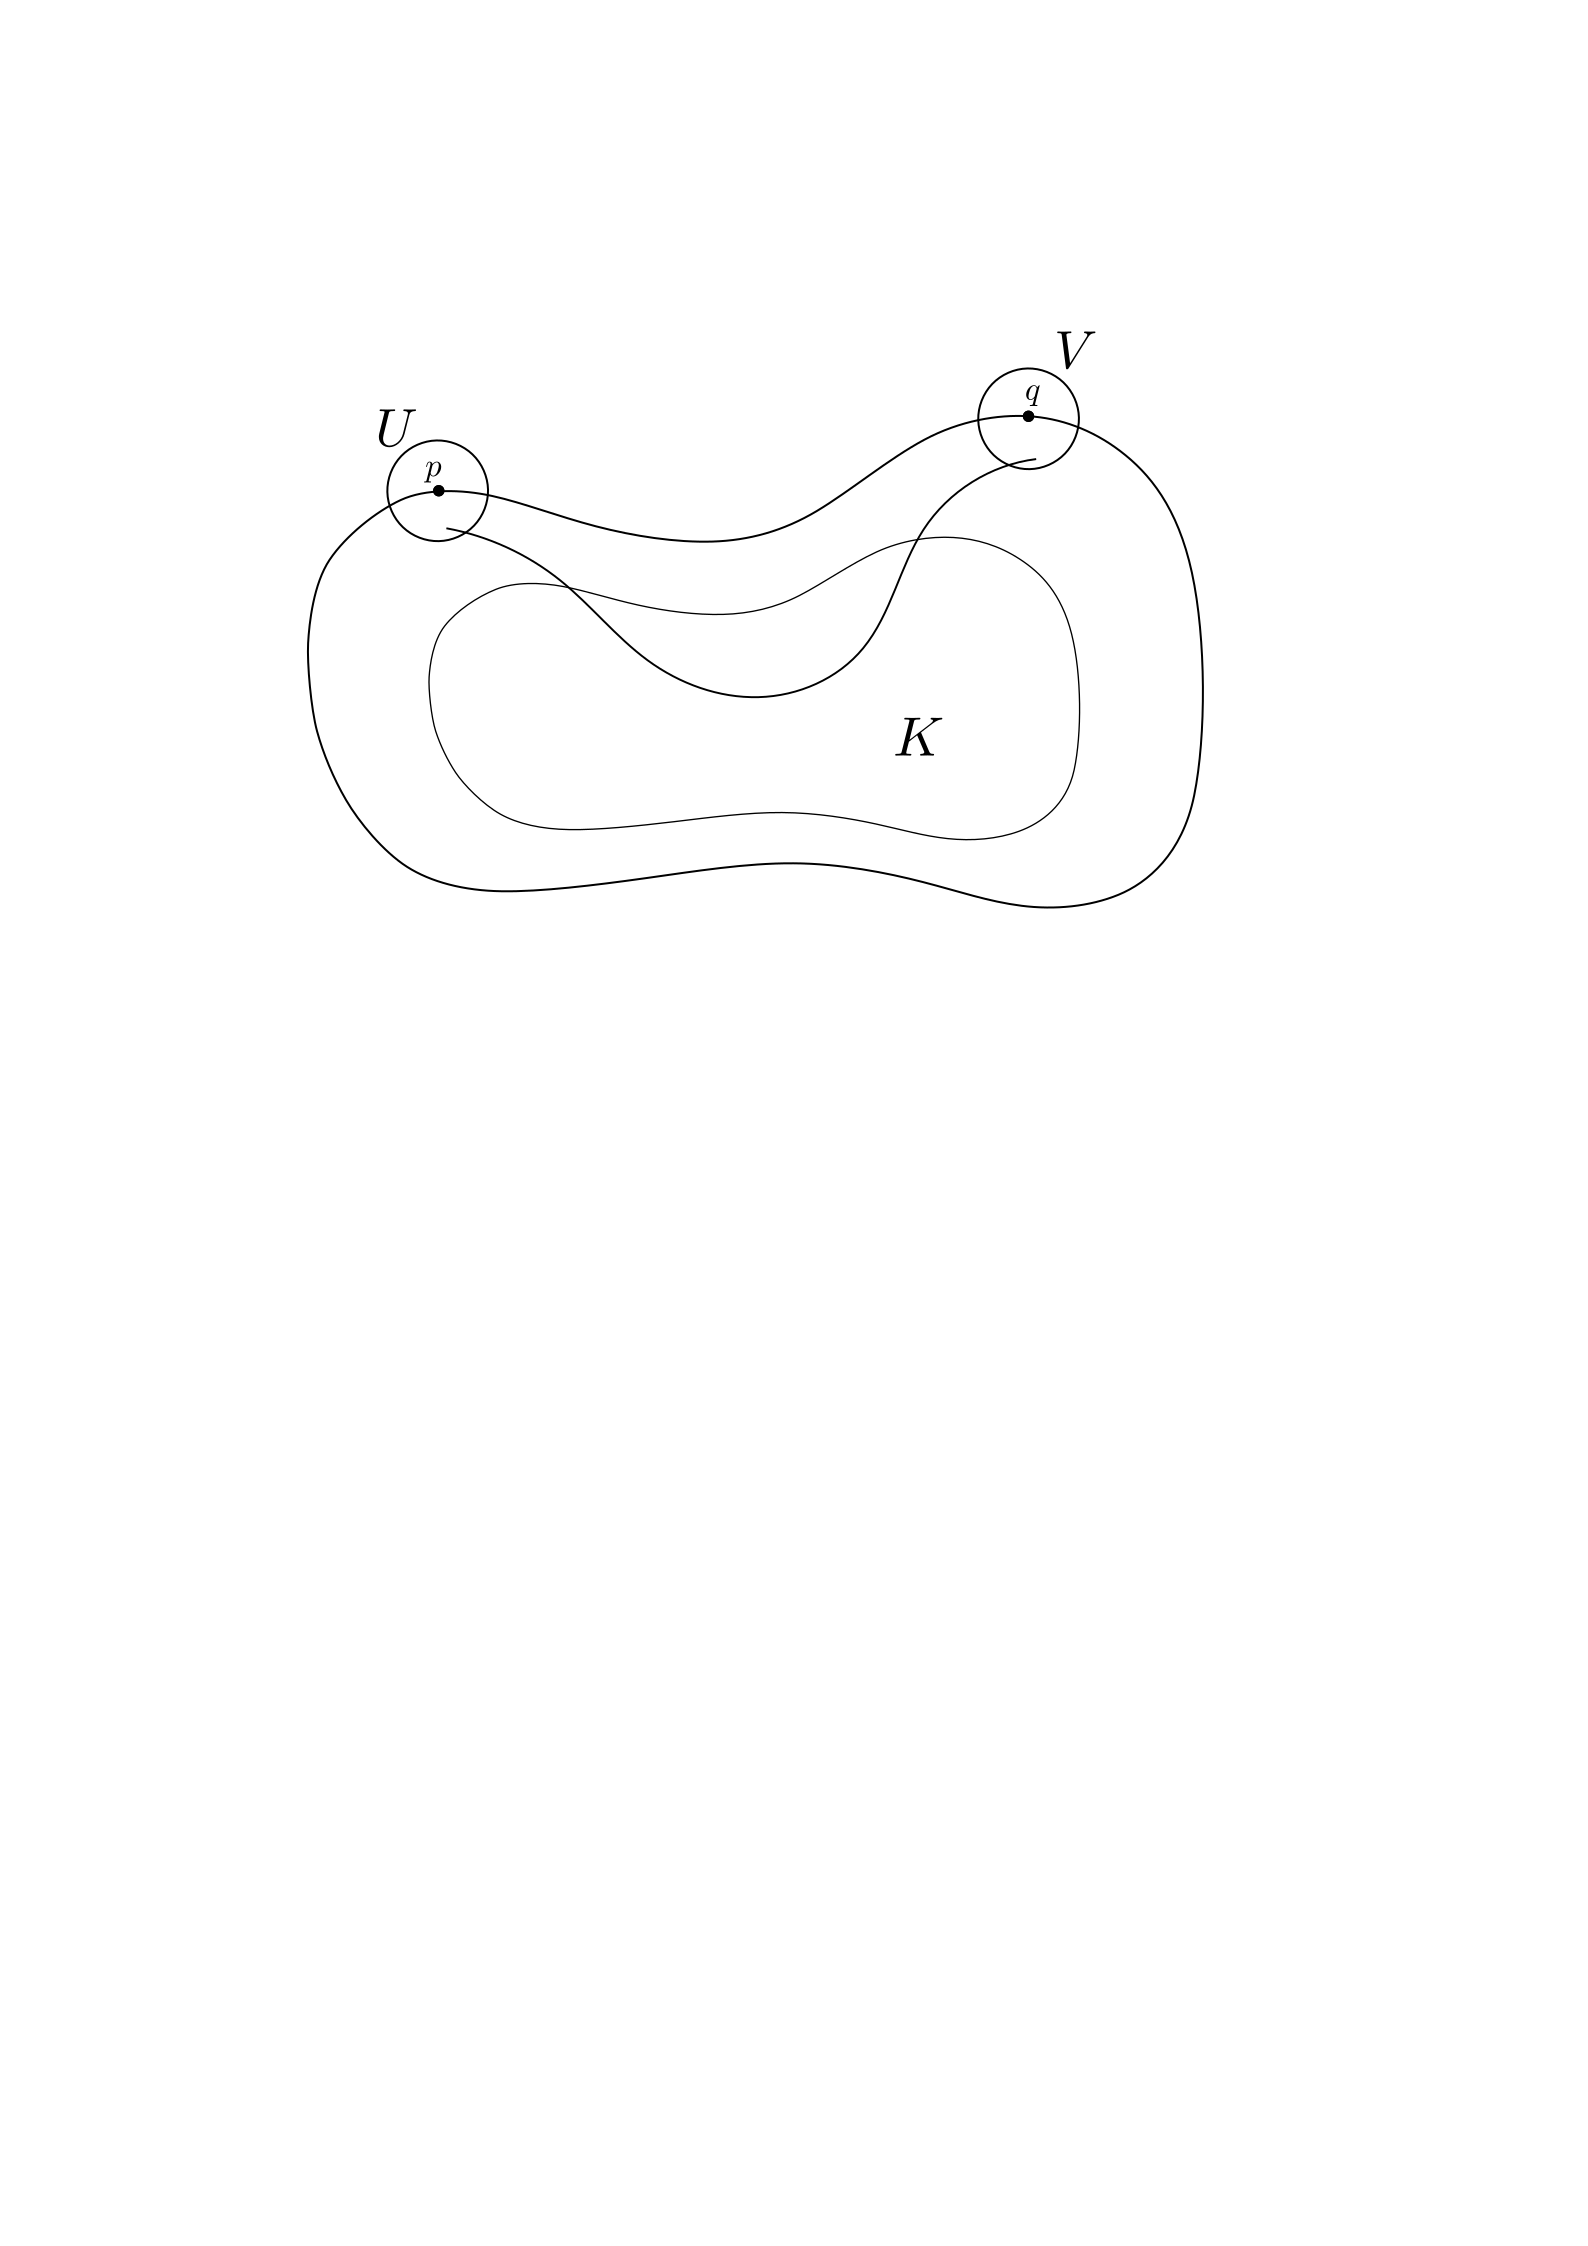
\includegraphics[width=1.05\textwidth, trim=0 16cm 0 3cm]{vis1.png}
    Condizione di visibilità: le simil-geodetiche ``curvano verso l'interno'', rimanendo dentro il compatto $K$.
  }
\end{frame}

\begin{frame}
  \frametitle{Un teorema di tipo ``Wolff-Denjoy'' per sottovarietà relativamente compatte}
  \only<1-2>{
    \begin{defn}
      Una varietà complessa $X$ si dice \textit{taut} se ogni funzione nella chiusura (rispetto alla topologia compatta-aperta) di $\text{Hol}(\mathbb{D},X)$ in $C^0(\mathbb{D},X^*)$ è in $\text{Hol}(\mathbb{D},X)$ oppure è la funzione costante $\infty$.
  \end{defn}\pause

    Si può dimostrare che ogni varietà taut è Kobayashi-iperbolica.
  }
  \only<3->{
    \begin{block}{Teorema (Chandel, Maitra, Sarkar, 2021; Bharali, Zimmer, 2022)}\begin{itshape}
      Sia $X$ una sottovarietà taut e relativamente compatta di una varietà complessa $Y$. \setcounter{beamerpauses}{3}\pause Supponiamo che esista un $\kappa_0>0$ tale che $X$ sia $(1,\kappa_0)$-visibile.
    
      Sia $F:X \longrightarrow X$ una funzione olomorfa. \pause Allora vale esattamente una delle seguenti affermazioni: \pause
      \begin{itemize}
        \item le orbite dei punti di $X$ tramite $F$ sono relativamente compatte in $X$; \pause oppure,
        \item esiste un unico punto di $\partial_YX$ tale che la successione delle iterate di $F$ converge, uniformemente sui compatti, a quel punto.
      \end{itemize}
    \end{itshape}\end{block}
  }
\end{frame}

\begin{frame}
  \frametitle{Un esempio di Bharali e Maitra: i domini Caltrops}
  \only<1-3>{
    \begin{defn}
      Un dominio limitato $\Omega\subseteq\mathbb{C}^n$, con $n\ge 2$, è detto \textit{dominio Caltrop} se esiste un insieme finito di punti $\{q_1,\dots,q_N\}\subseteq\partial\Omega$ tale che:\pause
      \begin{itemize}
          \item il sottoinsieme del bordo $\partial\Omega\setminus\{q_1,\dots,q_N\}$ è $C^2$ e $\Omega$ è strettamente pseudoconvesso in ogni punto di tale insieme;\pause
          \item per ogni $j=1,\dots, N$ esistono un intorno aperto e connesso $V_j\ni q_j$, due costanti $p_j\in(1,3/2)$ e $C_j>1$, una trasformazione unitaria $\mathbb{U}^{(j)}$ e una funzione continua $\psi_j:[0,A_j]\longrightarrow[0,+\infty)$, con $A_j>0$, tali che $\mathbb{U}_j(\Omega\cap V_j)$ è un ``solido di rivoluzione'':
      \end{itemize}
    \end{defn}
  }
  \only<4-9>{
    \begin{defn}
      \begin{equation*}\begin{split}
        \mathbb{U}_j(\Omega\cap V_j)=&\Bigg\{(z_1,\dots,z_n)\in\mathbb{C}^n\mid \mathfrak{Re}z_n\in (0,A_j),\\
        &(\mathfrak{Im}z_n)^2+\sum_{j=1}^{n-1}|z_j|^2<\psi_j(\mathfrak{Re}z_n)^2\Bigg\}
      \end{split}\end{equation*}
      dove $\mathbb{U}_j(z)=\mathbb{U}^{(j)}(z-q_j)$ per ogni $z\in\mathbb{C}^n$. \setcounter{beamerpauses}{4}\pause Inoltre, $\psi_j$ ha le seguenti proprietà:\pause
      \begin{itemize}
        \item è di classe $C^2$ su $(0,A_j)$;\pause
        \item per ogni $x\in[0,A_j]$ si ha $(1/C_j)x^{p_j} \le \psi_j(x) \le C_jx^{p_j}$;\pause
        \item si ha che $\psi_j$ è strettamente crescente e $\psi_j'$ è crescente su $(0,A_j)$;\pause
        \item si ha $\displaystyle\lim_{x\longrightarrow0^+}\psi_j(x)\psi_j''(x)=0$.
      \end{itemize}
    \end{defn}
  }
  \only<10>{
    \begin{figure}
      \begin{center}
          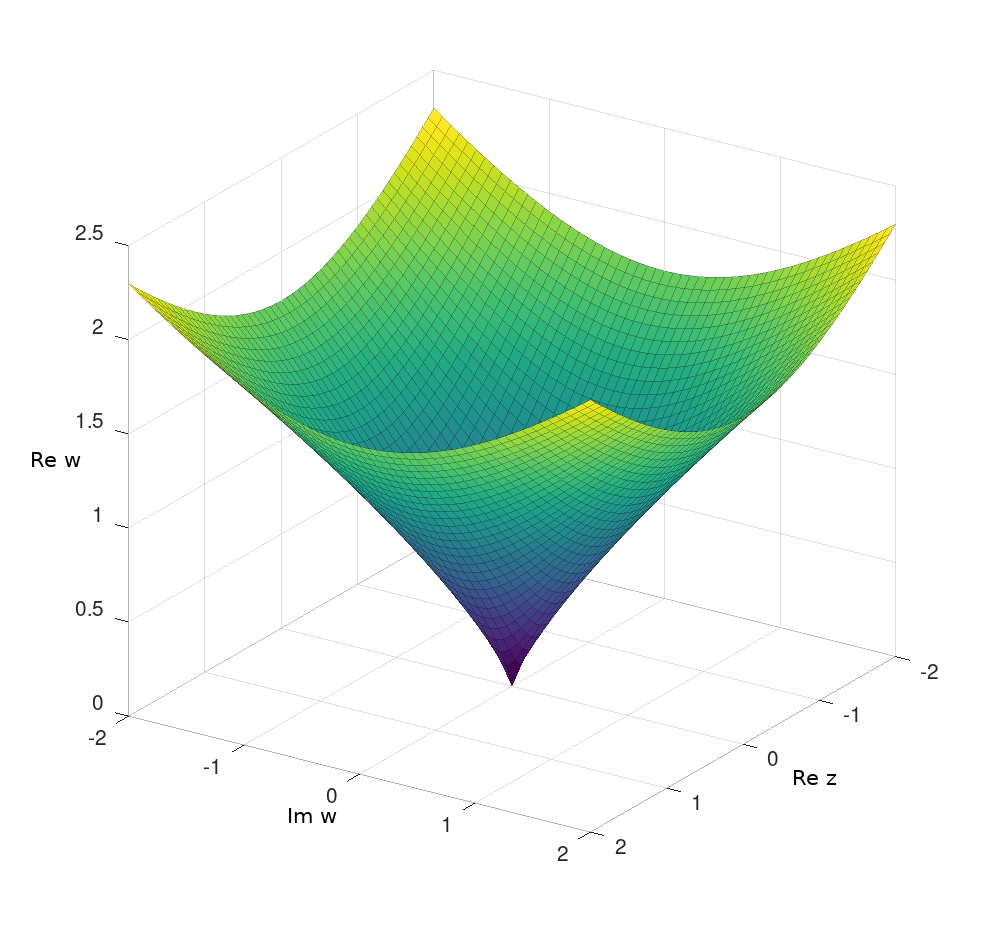
\includegraphics[width=0.65\textwidth, trim=0 4cm 0 1.7cm]{caltrop.png} \\
          \caption{proiezione a $\mathfrak{Im}z=0$ del bordo della punta in $\mathbb{C}^2$ con coordinate $(z,w)$ corrispondente a $\psi(x)=x^{5/4}$}
      \end{center}
  \end{figure}
  }
\end{frame}

\begin{frame}{Costruzione di un dominio Caltrop in $\mathbb{C}^2$}
  Siano $A,\beta>0$ e sia $\psi:[-A,\beta]\longrightarrow[0,+\infty)$ una funzione continua di classe $C^2$ su $(-A,\beta)$ tale che:\pause
  \begin{enumerate}
    \item per ogni $t\in(-A,-B)$ si ha $\psi(t)=(t+A)^p$;\pause
    \item per ogni $t\in(0,\beta)$ si ha $\psi(t)=\sqrt{\beta^2-t^2}$,
  \end{enumerate}
  dove $B\in(0,A)$ e $p\in(1,3/2)$. \pause Il dominio cercato è
  $$\Omega:=\{(z,w)\in\mathbb{C}^2\mid |z|^2+|\mathfrak{Im}w|^2<C\psi(\mathfrak{Re}w)^2,-A<\mathfrak{Re}w<\beta\},$$
  dove $C>0$ è una costante opportunamente scelta.\pause
  
  Le verifiche necessarie seguono da come è definita $\psi$; \pause per la pseudoconvessità, la funzione di definizione è
  $$\rho(z,w):=|z|^2+|\mathfrak{Im}w|^2-C\psi(\mathfrak{Re}w)^2.$$
\end{frame}

\begin{frame}[t]{I domini Caltrops sono $(\lambda,\kappa)$-visibili}
  \only<1-7>{
    Sia $\Omega$ un dominio limitato di $\mathbb{C}^d$. Poniamo
    $$M_\Omega(r):=\sup\left\{\frac{1}{K_\Omega(x;v)}\mid x\in\Omega,\delta_\Omega(x) \le r, \|v\|=1\right\},$$
    dove $\delta_\Omega$ indica la distanza da $\partial\Omega$.\pause
    \begin{thm}
      (Bharali, Maitra, 2021) Sia $\Omega$ un dominio limitato di $\mathbb{C}^d$. \setcounter{beamerpauses}{2}\pause Supponiamo che per esistano uno $z_0\in\Omega$ e una funzione $C^1$ strettamente crescente $f:(0,+\infty)\longrightarrow\mathbb{R}$, con $f(t)\longrightarrow+\infty$ per $t\longrightarrow+\infty$, tali che:\pause
      \begin{enumerate}
          \item si ha $k_\Omega(z_0,z) \le f\big(1/\delta_\Omega(z)\big)$ per ogni $z\in\Omega$;\pause
          \item si ha $M_\Omega(r)\longrightarrow 0$ per $r\longrightarrow 0$;\pause
          \item esiste $r_0>0$ tale che $\displaystyle\int_0^{r_0}\frac{M_\Omega(r)}{r^2}f'\left(\frac{1}{r}\right)\diff r<+\infty$.
      \end{enumerate}\pause
        
      Allora $\Omega$ è $(\lambda,\kappa)$-visibile per ogni $\lambda \ge 1$ e $\kappa>0$.
    \end{thm}
  }
  \only<8->{
    \begin{prop}
      I domini Caltrops sono $(\lambda,\kappa)$-visibili per ogni $\lambda\ge 1$ e $\kappa>0$.
    \end{prop}\setcounter{beamerpauses}{8}\pause
    \textit{Idea della dimostrazione:} si usa il teorema di Bharali e Maitra. Per vedere che un dominio Caltrop $\Omega$ ne soddisfa le ipotesi: \pause si calcola $k_D$ per un dominio planare $D$ usato come modello; \pause dopodiché si immergono copie di $D$ in $\Omega$ in maniera affine, di modo che ogni punto di $\Omega$ sufficientemente vicino al bordo sia contenuto in una di queste copie; \pause a questo punto, si usa il fatto che le funzioni olomorfe sono contrazioni per $k_X$ per stimare la distanza di Kobayashi su $\Omega$.
  }
\end{frame}

\begin{frame}{I domini Caltrop sono taut}
  \only<1->{
    \begin{lemma}
      Ogni varietà $X$ Kobayashi-iperbolica e $k_X$-completa è taut.
    \end{lemma}\pause
    \begin{lemma}
      Sia $\Omega\subseteq\mathbb{C}^n$ un dominio limitato tale che esiste uno $z_0\in\Omega$ tale che per ogni $\xi\in\partial\Omega$ si ha $\displaystyle\lim_{w\longrightarrow\xi}k_\Omega(z_0,w)=+\infty$; allora $(\Omega,k_\Omega)$ è completo.
    \end{lemma}\pause
    \begin{prop}
      I domini Caltrops sono taut.
    \end{prop}\pause
    \textit{Idea della dimostrazione:} Si usano i lemmi. Si distinguono due casi.\pause

    $\xi\in\partial\Omega\setminus\{q_1,\dots,q_N\}$: si usa la pseudoconvessità;\pause

    $\xi=q_j$ per $j=1,\dots,N$: si usa la forma di $\Omega$ vicino a $q_j$.
  }
\end{frame}

\begin{frame}
  \frametitle{Strada per la dimostrazione del teorema di tipo ``Wolff-Denjoy''}
  \begin{enumerate}
    \item dall'ipotesi che la varietà sia taut, per un teorema di Abate segue che se le orbite non sono relativamente compatte allora la successione delle iterate è compattamente divergente;\pause
    \item dalle ipotesi di visibilità e di relativa compattezza segue, a meno di sottosuccessioni, la convergenza uniforme sui compatti a una costante nel bordo della varietà;\pause
    \item sempre per la condizione di visibilità, tale limite è lo stesso per ogni sottosuccessione, dunque dev'essere il limite di tutta la successione.
  \end{enumerate}
\end{frame}

\begin{frame}[t]
  \frametitle{Dimostrazione dell'estensione al bordo}
  \only<1->{
  \begin{cor}
    Siano $\Omega_1, \Omega_2 \subseteq \mathbb{C}^n$ domini limitati e strettamente pseudoconvessi, e sia $f:\Omega_1 \longrightarrow \Omega_2$ una funzione olomorfa propria. Allora $f$ si estende con continuità a $\bar{f}:\overline{\Omega}_1\longrightarrow\overline{\Omega}_2$ tale che $\bar{f}(\partial\Omega_1)\subseteq\partial\Omega_2$ e la restrizione al bordo è lipschitziana rispetto alle distanze di Carnot-Carathéodory sui bordi.
  \end{cor}
  }
  \only<2-3>{
  \textit{Traccia della dimostrazione:} siano $d_1,d_2$ le distanze di Kobayashi su $\Omega_1, \Omega_2$, allora per ogni $x,y \in \Omega_1$ si ha
  $$d_2\big(f(x),f(y)\big)\le d_1(x,y);$$
  }
  \only<3>{
  inoltre, poiché $f$ è propria esiste $C_1 \ge 1$ tale che per ogni $x \in \Omega_1$ abbiamo
  $$\delta_1(x)/C_1 \le \delta_2\big(f(x)\big) \le C_1\delta_1(x),$$
  dove $\delta_j$ è la distanza dal bordo in $\Omega_j$.
  }
  \only<4->{
  Mettendo assieme queste due disuguaglianze e il Teorema, dette $d_H^j$ le rispettive distanze di Carnot-Carathéodory, troviamo che esiste $C_2 \ge 0$ tale che per ogni $x,y \in \Omega_1$ si ha
  $$d_H^2\Big(\pi\big(f(x)\big),\pi\big(f(y)\big)\Big) \le C_2\Big(d_H^1\big(\pi(x),\pi(y)\big)+\max\{\delta_1^{1/2}(x),\delta_1^{1/2}(y)\}\Big).$$
  }
  \only<5>{Utilizzando queste disuguaglianze, si dimostra la tesi. \qed}
\end{frame}

\begin{frame}
  \frametitle{Fine}
  \begin{center}
    \LARGE Grazie per l'attenzione!
  \end{center}
\end{frame}


\end{document}
